%%%%%%%%%%%%%%%%%%%%%%%%%%%%%%%%%%%%%%%%%
% Beamer Presentation
% LaTeX Template
% Version 1.0 (10/11/12)
%
% This template has been downloaded from:
% http://www.LaTeXTemplates.com
%
% License:
% CC BY-NC-SA 3.0 (http://creativecommons.org/licenses/by-nc-sa/3.0/)
%
%%%%%%%%%%%%%%%%%%%%%%%%%%%%%%%%%%%%%%%%%

%----------------------------------------------------------------------------------------
%	PACKAGES AND THEMES
%----------------------------------------------------------------------------------------

\documentclass{beamer}

\mode<presentation> {

% The Beamer class comes with a number of default slide themes
% which change the colors and layouts of slides. Below this is a list
% of all the themes, uncomment each in turn to see what they look like.

%\usetheme{default}
%\usetheme{AnnArbor}
%\usetheme{Antibes}
%\usetheme{Bergen}
%\usetheme{Berkeley}
%\usetheme{Berlin}
%\usetheme{Boadilla}
%\usetheme{CambridgeUS}
%\usetheme{Copenhagen}
%\usetheme{Darmstadt}
%\usetheme{Dresden}
%\usetheme{Frankfurt}
%\usetheme{Goettingen}
%\usetheme{Hannover}
%\usetheme{Ilmenau}
%\usetheme{JuanLesPins}
%\usetheme{Luebeck}
\usetheme{Madrid}
%\usetheme{Malmoe}
%\usetheme{Marburg}
%\usetheme{Montpellier}
%\usetheme{PaloAlto}
%\usetheme{Pittsburgh}
%\usetheme{Rochester}
%\usetheme{Singapore}
%\usetheme{Szeged}
%\usetheme{Warsaw}

% As well as themes, the Beamer class has a number of color themes
% for any slide theme. Uncomment each of these in turn to see how it
% changes the colors of your current slide theme.

%\usecolortheme{albatross}
%\usecolortheme{beaver}
%\usecolortheme{beetle}
%\usecolortheme{crane}
%\usecolortheme{dolphin}
%\usecolortheme{dove}
%\usecolortheme{fly}
%\usecolortheme{lily}
%\usecolortheme{orchid}
%\usecolortheme{rose}
%\usecolortheme{seagull}
%\usecolortheme{seahorse}
%\usecolortheme{whale}
%\usecolortheme{wolverine}

%\setbeamertemplate{footline} % To remove the footer line in all slides uncomment this line
%\setbeamertemplate{footline}[page number] % To replace the footer line in all slides with a simple slide count uncomment this line

%\setbeamertemplate{navigation symbols}{} % To remove the navigation symbols from the bottom of all slides uncomment this line
}

\usepackage{graphicx} % Allows including images
\usepackage{booktabs} % Allows the use of \toprule, \midrule and \bottomrule in tables
\usepackage{multimedia}
\usepackage{blkarray}
\usepackage{kbordermatrix}
\renewcommand{\kbldelim}{[}% Left delimiter
\renewcommand{\kbrdelim}{]}% Right delimiter

%----------------------------------------------------------------------------------------
%	TITLE PAGE
%----------------------------------------------------------------------------------------

\title[Music Making]{Music Making Using Markov Chains} % The short title appears at the bottom of every slide, the full title is only on the title page

\author{Peng Zhao, Chengying Wang, and Andrew Pak} % Your name
\institute[SC] % Your institution as it will appear on the bottom of every slide, may be shorthand to save space
{
Swarthmore College \\ % Your institution for the title page
\medskip
\textit{} % Your email address
}
\date{\today} % Date, can be changed to a custom date

\begin{document}

\begin{frame}
\titlepage % Print the title page as the first slide
\end{frame}

\begin{frame}
\frametitle{Overview} % Table of contents slide, comment this block out to remove it
\tableofcontents % Throughout your presentation, if you choose to use \section{} and \subsection{} commands, these will automatically be printed on this slide as an overview of your presentation
\end{frame}

%----------------------------------------------------------------------------------------
%	PRESENTATION SLIDES
%----------------------------------------------------------------------------------------

%------------------------------------------------
\section{Introduction} % Sections can be created in order to organize your presentation into discrete blocks, all sections and subsections are automatically printed in the table of contents as an overview of the talk
%------------------------------------------------

\subsection{Why music making?} % A subsection can be created just before a set of slides with a common theme to further break down your presentation into chunks
\begin{frame}
\frametitle{Why Music Making?}
\begin{itemize}
\item There are distinct states, classified as notes, that are easy to model
\item We have existing models of "good" music to build our transition matrix
\item We can recreate a song randomly from this "good" transition matrix.
\end{itemize}
\end{frame}

\begin{frame}
\frametitle{How We Did It}
\begin{itemize}
\item There exists a online database storing are of MIDI files
\item MIDI files basically break down musical notes into 3 categories
\begin{itemize}
\item Tick - description of tick
\item Pitch - description of pitck
\item Velocity - description of velocity
\end{itemize}
\item Used this representation of music to create transition probabilities for each of these categories
\end{itemize}
\end{frame}

\section{Transition Matrices}
\begin{frame}
\frametitle{Transition Matrices}
\begin{itemize}
\item Length Matrix - We combined different elements of the tick characteristic here
\item Pitch Matrix
\item Velocity Matrix
\end{itemize}
\end{frame}

\subsection{Length Matrix}

\begin{frame}
\frametitle{Length Matrix}
Insert our transition matrix Here
\end{frame}

\subsection{Pitch Matrix}
\begin{frame}
\frametitle{Length Matrix}
\begin{figure}
 \[  \kbordermatrix{
 	&\text{Length 1} & \text{L2}& & \text{L128}\\
 	\text{Length1 }&m_1 		& 0 		&\cdots 	&0\\
	\text{L2}&0		& m_2 	&		&\vdots\\
		&\vdots 		&&\ddots	&0\\
	\text{L128}&0		& \cdots 	& 0 		& m_i
	}
\]
%\includegraphics[width=0.8\linewidth]{test}
\end{figure}
\end{frame}


\subsection{Velocity Matrix}
\begin{frame}
\frametitle{Velocity Matrix}
\begin{figure}
\[
  \kbordermatrix{
    & c_1 & c_2 & c_3 & c_4 & c_5 &c_6 \\
    r_1 & 1 & 1 & 1 & 1 & 1 &0\\
    r_2 & 0 & 1 & 0 & 0 & 1 &0\\
    r_3 & 0 & 0 & 1 & 0 & 1 &0\\
    r_4 & 0 & 0 & 0 & 1 & 1 &0\\
    r_5 & 0 & 0 & 0 & 0 & 1 &0
  }
\]
\end{figure}
\end{frame}

\begin{frame}
	\frametitle{One way of visualization}
	\begin{itemize}
	\item Visualization of our MC with 3 ticks, pitches, and velocities
	\end{itemize}
	\begin{figure}
		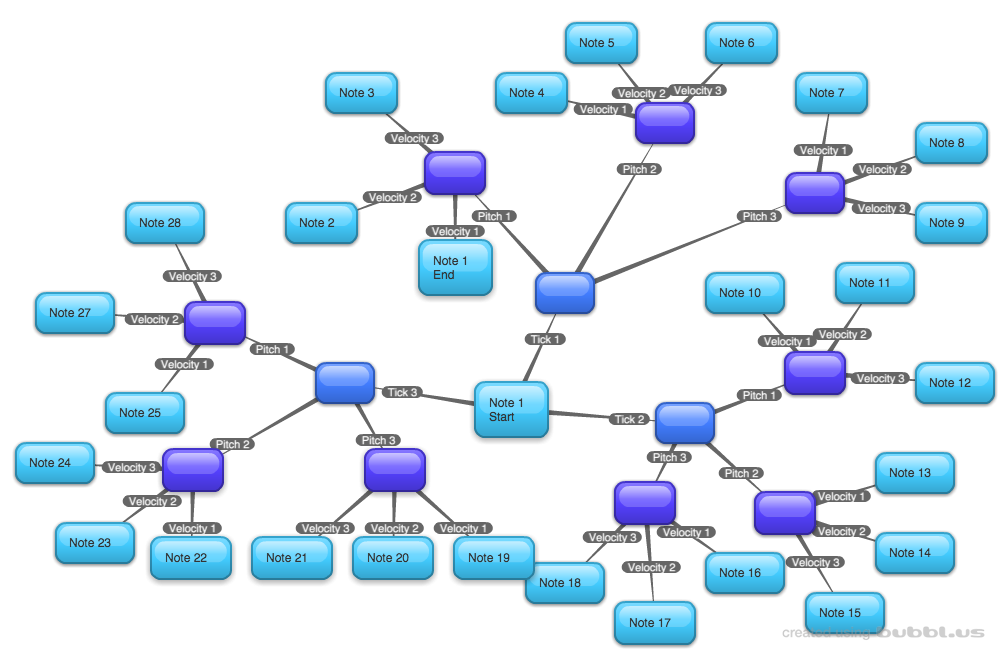
\includegraphics[scale = 0.3]{matrixViz}
	\end{figure}
\end{frame}

\section{Examples}
\begin{frame}
	\frametitle{Simulation?}
\end{frame}
\begin{frame}
	\frametitle{Examples}
	\sound[autostart, label = andrew]{}{"midis/haydnNew.mid"}
	\hyperlinksound[mixsound = false]{andrew}{hayden.mid}
\end{frame}



\begin{frame}
\frametitle{Acknowledgements}
We acknowledge all who helped us participate on this thingy. Thank you very much
\end{frame}

%------------------------------------------------

%------------------------------------------------


%------------------------------------------------



%------------------------------------------------

%------------------------------------------------

%------------------------------------------------


%------------------------------------------------



%------------------------------------------------

%\begin{frame}[fragile] % Need to use the fragile option when verbatim is used in the slide
%\frametitle{Citation}
%An example of the \verb|\cite| command to cite within the presentation:\\~

%This statement requires citation \cite{p1}.
%\end{frame}

%------------------------------------------------

\begin{frame}
\frametitle{References}
\footnotesize{
\begin{thebibliography}{99} % Beamer does not support BibTeX so references must be inserted manually as below
\bibitem[Smith, 2012]{p1} John Smith (2012)
\newblock Title of the publication
\newblock \emph{Journal Name} 12(3), 45 -- 678.
\end{thebibliography}
}
\end{frame}

%------------------------------------------------

\begin{frame}
\Huge{\centerline{The End}}
\end{frame}

%----------------------------------------------------------------------------------------

\end{document} 